%-----------------------------------------------------------------------------------------------
\makeatletter
\immediate\write18{datelog > \jobname.info} % site script for $(date '+%Y-%m-%d %Hh%Mm%Ss')
\makeatother
%-----------------------------------------------------------------------------------------------
%-----------------------------------------------------------------------------------------------
\usetheme{Copenhagen}
\usepackage{beamercolorthemeUTF2}
\usefonttheme{serif}
%-----------------------------------------------------------------------------------------------
\usepackage[utf8]{inputenc}
\usepackage[greek,french,english,brazil]{babel} % last becomes the active one
\usepackage{pslatex}
\usepackage{amssymb,amsmath}
\usepackage{soul}
\usepackage[squaren,Gray,cdot]{SIunits}
\usepackage[nice]{nicefrac}
\usepackage{tikz}
\usepackage{amscd}
\usepackage{stmaryrd}
\usepackage{scalerel}
\usepackage{xspace}
%-----------------------------------------------------------------------------------------------


%-----------------------------------------------------------------------------------------------
%-----------------------------------------------------------------------------------------------
% Mathematical
%-----------------------------------------------------------------------------------------------
\newcommand{\vet}[1]{\underline{{#1}}}
\newcommand{\mat}[1]{\underline{\underline{{#1}}}}
\newcommand{\cub}[1]{\underline{\underline{\underline{{#1}}}}}
\newcommand{\eqdef}{{\ensuremath\stackrel{\text{\tiny def}}{=}}}
%-----------------------------------------------------------------------------------------------
% Linguistic
%-----------------------------------------------------------------------------------------------
\newcommand{\GRtxt}[1]{\begin{otherlanguage}{greek}{{#1}}\end{otherlanguage}}
\newcommand{\FRtxt}[1]{\begin{otherlanguage}{french}{{#1}}\end{otherlanguage}}
%-----------------------------------------------------------------------------------------------
% Presentation
%-----------------------------------------------------------------------------------------------
\newcommand{\BkgImgH}[1]{% Places an image centered on the slide background filling the height
    \usebackgroundtemplate{\parbox{\paperwidth}{%
        \vspace*{1sp}\centering\includegraphics[height=\paperheight]{{#1}}
}}}
\newcommand{\BkgImgW}[1]{% Places an image centered on the slide background filling the width
    \usebackgroundtemplate{\parbox{\paperwidth}{%
        \vspace*{1sp}\centering\includegraphics[width=\paperwidth]{{#1}}
}}}
\newcommand{\ArtEndH}[3]{% Transitions to plain image (last) slide: #1:prefix #2,#3:extensions
    \BkgImgH{root/../art/#1.#2}
    \frame<handout:0>[plain]{%
        \transdissolve\vspace*{72mm}\color{white}\scriptsize\bf\input{root/../art/#1.#3}}
    \usebackgroundtemplate{\mbox{~}}
}
\newcommand{\ArtEndW}[3]{% Transitions to plain image (last) slide: #1:prefix #2,#3:extensions
    \BkgImgW{root/../art/#1.#2}
    \frame<handout:0>[plain]{%
        \transdissolve\vspace*{72mm}\color{white}\scriptsize\bf\input{root/../art/#1.#3}}
    \usebackgroundtemplate{\mbox{~}}
}
\newcommand{\ImgColW}[3]{% Inserts a full-width image in a column
    \includegraphics[width=\columnwidth]{root/../art/#1.#2}\\[-0.5\baselineskip]
    \parbox{\columnwidth}{\tiny\hfill\scalebox{0.85}{\input{root/../art/#1.#3}}}
}
\newcommand{\txtpic}[1]{%
    \fcolorbox{lightgray}{white!90!black}{{#1}} 
}
%-----------------------------------------------------------------------------------------------


%-----------------------------------------------------------------------------------------------
\newcommand{\VPMS}{{\ensuremath V_{\mathrm{PMS}}}}
\newcommand{\VPMI}{{\ensuremath V_{\mathrm{PMI}}}}
%-----------------------------------------------------------------------------------------------
\title{C.01.01 -- Ciclo Otto de Tempo Finito de Adição de Calor}
\subtitle{FTHA -- Finite-Time Heat Addition Otto Engine Model}
\author{Prof.~C.~Naaktgeboren, PhD}
\date{{\scriptsize\tt%
    
\includegraphics[height=6.0mm]{root/00-res/cc/by-nc-nd-88x31.pdf}\\[\smallskipamount]
    https://github.com/CNThermSci/ApplThermSci\\
    Compiled on \input{\jobname.info}
}}
%-----------------------------------------------------------------------------------------------
\begin{document}
%-----------------------------------------------------------------------------------------------
\logo{%
    \parbox{158mm}{% There's a 1mm gap on each side of the 160mm x 90mm slide logo line
        
\includegraphics[height=6.5mm]{root/00-res/UTFPR/UTFPR-logo-A.pdf}\hfill%
        
\includegraphics[height=6.5mm]{root/00-res/logo/CNThermSci-logo-A.pdf}%
%   \parbox{126mm}{% There's a 1mm gap on each side of the 128mm x 96mm slide logo line
%       
\includegraphics[height=6.0mm]{root/00-res/UTFPR/UTFPR-logo-A.pdf}\hfill%
%       
\includegraphics[height=6.0mm]{root/00-res/logo/CNThermSci-logo-A.pdf}%
}} % Alpha logos
%-----------------------------------------------------------------------------------------------
\frame{\titlepage}
%-----------------------------------------------------------------------------------------------

%-----------------------------------------------------------------------------------------------
\frame{\tableofcontents}
%-----------------------------------------------------------------------------------------------

    % !j 96 -i8
    %-------------------------------------------------------------------------------------------
    \begin{frame}{Melhorando o Ciclo Otto Ideal}\vspace*{-2em}
        \uncover<1->{O ciclo Otto \alert{ideal}, da termodinâmica aplicada:}
        \begin{columns}
        \column{0.50\textwidth}
        \begin{itemize}
            \item<2->  Assume todas as \alert{hipóteses padrão a ar};
            \item<8->  Assume entrada de calor \alert{isocórica};
            \item<9->  Possui parâmetros \alert{$r$} e \alert{$k$}, e
            \item<10-> Solução analítica, \alert{hip.~padrão a ar frio}:\\[\bigskipamount]
        \end{itemize}
        \begin{equation*}
            \uncover<12->{\alert{\eta_t = 1 - r^{1-k}}\quad\rightharpoondown}
        \end{equation*}%
        \vspace*{-1em}
        \begin{itemize}
            \item<13-> $\eta_t\!:\!\eta_t(r, k)$ \alert{apenas}!
        \end{itemize}
        \column{0.50\textwidth}
        \begin{itemize}
            \item<3->  Gás \alert{ideal};
            \item<4->  Processos \alert{internamente reversíveis};
            \item<5->  Entrada de \alert{calor} modela a combustão;
            \item<6->  Saída de \alert{calor} modela a exaustão;
            \item<7->  Modelo em \alert{ciclo fechado};
            \item<11-> Calores específicos \alert{constantes}.
        \end{itemize}
        \end{columns}
    \end{frame}
    %-------------------------------------------------------------------------------------------

    % !j 96 -i8
    %-------------------------------------------------------------------------------------------
    \begin{frame}{Desvios do ciclo Otto ideal---incluem, mas não limitados a:}\vspace*{-2em}
        \begin{center}
            \includegraphics[height=40mm,width=60mm]{%
                fig/P-V_diagram_deviations_to_Otto_cycle.pdf}\\
            \footnotesize  Diagrama  $P-V$  ilustrativo  de   perdas   por   (i)~combustão   não
                instantânea---verde,    (ii)~transferência    de     calor---vermelho---e     de
                (iii)~bombeamento---azul. Fonte: adaptado de Wikimedia Commons.
            {\tiny\tt https://upload.wikimedia.org/wikipedia/commons/6/6c/P-V\_diagram\_deviations\_to\_Otto\_cycle.svg.}
        \end{center}
    \end{frame}
    %-------------------------------------------------------------------------------------------

    % !j 96 -i8
    %-------------------------------------------------------------------------------------------
    \begin{frame}{Ciclo Otto padrão a ar de tempo finito de adição de calor---FTHA}\vspace*{-2em}
        \begin{itemize}
            \item<1->  Modela combustão (adição de calor) de forma \alert{não instantânea}:
            \begin{itemize}
                \item<2->  Interações \alert{simultâneas} de \alert{calor} e \alert{trabalho};
                \item<3->  Tempos de motor \alert{discretizados} em \alert{sub-processos};
                \item<4->  Elemento computacional: sub-processo \alert{localmente politrópico}.
            \end{itemize}
            \item<5->  Mantém-se como modelo \alert{padrão a ar}:
            \begin{itemize}
                \item<6->  Transferência de calor para bloco inclui \alert{irreversibilidades};
                \item<7->  Perdas de bombeamento envolvem \alert{sistema e ciclo abertos}.
            \end{itemize}
            \item<8->  Mantém-se como modelo de \alert{substância pura}:
            \begin{itemize}
                \item<9->  Evita \alert{combustão e equilíbrio químico};
                \item<10-> Evita modelagem termodinâmica de \alert{misturas reativas}.
            \end{itemize}
        \end{itemize}
    \end{frame}
    %-------------------------------------------------------------------------------------------

    % !j 96 -i8
    %-------------------------------------------------------------------------------------------
    \begin{frame}{Ciclo Otto padrão a ar de tempo finito de adição de calor---FTHA}\vspace*{-2em}
        \begin{itemize}
            \item<1->  Inclui todos os parâmetros do \alert{ciclo Otto ideal}:
            \begin{itemize}
                \item<2->  \alert{Razão de compressão} do motor;
                \item<3->  \alert{Calores específicos} do fluido de trabalho.
            \end{itemize}
            \item<4->  Inclui parâmetros \alert{construtivos} do \alert{motor}:
            \begin{itemize}
                \item<5->  Conjunto \alert{pistão-cilindro};
                \item<6->  Mecanismo \alert{biela-manivela}.
            \end{itemize}
            \item<7->  Inclui parâmetros \alert{operacionais} do \alert{motor}:
            \begin{itemize}
                \item<8->  \alert{Velocidade angular} (rotação);
                \item<9->  Ângulo de \alert{ignição} e
                \item<10-> \alert{Duração da combustão}.
            \end{itemize}
        \end{itemize}
    \end{frame}
    %-------------------------------------------------------------------------------------------

%-----------------------------------------------------------------------------------------------
\section{Modelagem do Motor}
%-----------------------------------------------------------------------------------------------

%-----------------------------------------------------------------------------------------------
\subsection{Mecanismo Biela-Manivela}
%-----------------------------------------------------------------------------------------------

    % !j 96 -i8
    %-------------------------------------------------------------------------------------------
    \begin{frame}{Parâmetros do mecanismo}\vspace*{-2em}
        \begin{columns}
        \column{0.50\textwidth}
        \begin{itemize}
            \item<1-> \alert{Diâmetro} do pistão/cilindro, \alert{$D$};
            \item<2-> \alert{Raio} da manivela, \alert{$R$};
            \item<3-> \alert{Curso} do pistão, \alert{$S = 2R$};
            \item<4-> \alert{Comprimento} da biela, \alert{$L$};
            \item<5-> \alert{Volume} morto (do PMS), \alert{$\VPMS$};
            \item<6-> \alert{Posição} do pistão (rel.~PMS), \alert{$x$};
            \item<7-> \alert{Volume} máximo (do PMI), \alert{$\VPMI$};
            \item<8-> \alert{Razão de compressão}, \alert{$r = \dfrac{\VPMS}{\VPMI}$}.
        \end{itemize}
        \column{0.50\textwidth}
        \begin{center}
            \uncover<1->{\vspace*{-5mm}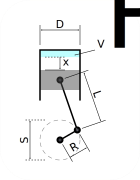
\includegraphics[height=70.0mm]{fig/FTHAEngine01.pdf}}
        \end{center}
        \end{columns}
    \end{frame}
    %-------------------------------------------------------------------------------------------

    % !j 96 -i8
    %-------------------------------------------------------------------------------------------
    \begin{frame}{Parâmetros do mecanismo}\vspace*{-2em}
        \begin{columns}
        \column{0.50\textwidth}
        \begin{itemize}
            \item<1-> \alert{Diâmetro} do pistão/cilindro, \alert{$D$};
            \item<2-> \alert{Raio} da manivela, \alert{$R$};
            \item<3-> \alert{Curso} do pistão, \alert{$S = 2R$};
            \item<4-> \alert{Comprimento} da biela, \alert{$L$};
            \item<5-> \alert{Volume} morto (do PMS), \alert{$\VPMS$};
            \item<6-> \alert{Posição} do pistão (rel.~PMS), \alert{$x$};
            \item<7-> \alert{Volume} máximo (do PMI), \alert{$\VPMI$};
            \item<8-> \alert{Razão de compressão}, \alert{$r = \dfrac{\VPMS}{\VPMI}$}.
        \end{itemize}
        \column{0.50\textwidth}
        \begin{center}
            \uncover<1->{\vspace*{-5mm}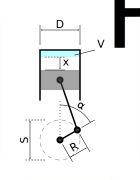
\includegraphics[height=70.0mm]{fig/FTHAEngine02.pdf}}
        \end{center}
        \end{columns}
    \end{frame}
    %-------------------------------------------------------------------------------------------

    % !j 96 -i8
    %-------------------------------------------------------------------------------------------
    \begin{frame}{Título}\vspace*{-2em}
        \begin{columns}
        \column{0.50\textwidth}
        \uncover<1->{Um \alert{template} de slide.}
        \column{0.50\textwidth}
        \uncover<2->{De \alert{duas} colunas.}
        \end{columns}
    \end{frame}
    %-------------------------------------------------------------------------------------------

%-----------------------------------------------------------------------------------------------
\subsection{Tempos (\emph{Timings}) do Motor}
%-----------------------------------------------------------------------------------------------

    % !j 96 -i8
    %-------------------------------------------------------------------------------------------
    \begin{frame}{Título}\vspace*{-2em}
        \uncover<1->{Um \alert{template} de slide.}
    \end{frame}
    %-------------------------------------------------------------------------------------------

%-----------------------------------------------------------------------------------------------
\section{Modelagem do Ciclo}
%-----------------------------------------------------------------------------------------------

%-----------------------------------------------------------------------------------------------
\subsection{Modelo de Substância}
%-----------------------------------------------------------------------------------------------

    % !j 96 -i8
    %-------------------------------------------------------------------------------------------
    \begin{frame}{Título}\vspace*{-2em}
        \uncover<1->{Um \alert{template} de slide.}
    \end{frame}
    %-------------------------------------------------------------------------------------------

%-----------------------------------------------------------------------------------------------
\subsection{Procedimento de Solução}
%-----------------------------------------------------------------------------------------------

    % !j 96 -i8
    %-------------------------------------------------------------------------------------------
    \begin{frame}{Título}\vspace*{-2em}
        \uncover<1->{Um \alert{template} de slide.}
    \end{frame}
    %-------------------------------------------------------------------------------------------

%-----------------------------------------------------------------------------------------------
\section{Tópicos de Leitura}
%-----------------------------------------------------------------------------------------------

    %------------------------------------------------------------------------------------------
    \begin{frame}[allowframebreaks]{Tópicos de Leitura}
        \begin{thebibliography}{Çengel, Y.~A., 2013}
            \bibitem[Çengel, Y.~A., 2013]{2013-CengelYA+BolesMA-AMGH}
                Çengel, Y.~A. e Boles, M.~A.
                \newblock{%
                    {\em Termodinâmica $7^\mathrm{a}\!$ Edição\/}.
                    \alert{Seções~9--3 a 9--5.}
                }
                \newblock{\footnotesize AMGH. Porto Alegre. ISBN 978-85-8055-200-3.}
            \bibitem[Naaktgeboren, C., 2016]{2017-NaaktgeborenC-IntJMechEngEduc}
                Naaktgeboren, C.
                \newblock{%
                    {\em An air-standard finite-time heat addition Otto engine model\/}.
                }
                \newblock{\alert{Int.~J.~Mech.~Eng.~Educ. 45 (2), 2017.}}
                \newblock{\footnotesize DOI 10.1177/0306419016689447.}
        \end{thebibliography}
    \end{frame}
    %------------------------------------------------------------------------------------------

    % Finishes with stunning image, with credit
    \ArtEndW{horizon-768759_1280}{jpg}{txt}

%-----------------------------------------------------------------------------------------------
\end{document}
%-----------------------------------------------------------------------------------------------

